\section{Aufbau und Versuchsdurchführung}

Während des gesamten Versuches wird eine Ultraschallsonde mit $\SI{2}{\mega\hertz}$ verwendet. Diese Ultraschallsonde ist an ein Echoskop angeschlossen, dabei kann zwischen den Einstellungen
\enquote{REFLEC.} und \enquote{TRANS.} umgestellt werden. Im folgenden wurden nur Messungen im Impuls-Echo-Verfahren durchgeführt, wie in Abb ... gezeigt, somit wurde der Regler zu Beginn auf \enquote{REFLEC.}
geschaltet und dort gelassen. Das Echoskop wird nun mit einem Computer verbunden und die Daten lassen sich über das Programm \enquote{A-Scan} auslesen.

\subsection{Messungen am Acrylblock}

Zur Untersuchung der Schallgeschwindigkeit in Acryl wird ein Acrylblock mit elf Fehlstellen verwendet. Dabei lassen sich die Geschwindigkeit, sowie die jeweiligen Laufstrecken aus der gemessenen Laufzeit ermitteln. Eine schematische Darstellung 
des Acrylblock ist in Abbildung \ref{fig:skizzeyo} dargestellt. Dabei stellen die Größen $A$ bis $K$ die Fehlstellen innerhalb des Acryls im Augenmaß dar. Die eingezeichneten Längen, also von $A'$ bis $K''$, wurden zunächst mit einer Schieblehre ausgemessen. Der Acrylblock wird während der Messung auf ein Papiertuch gelegt um Kratzer zu vermeiden und 
nun wird Ultraschallgel auf das Acrylstück aufgetragen. Anschließend werden über die Ultraschallsonde die einzelnen Fehlstellen detektiert, dies geschieht über die Impuls-Echo-Methode und es entsteht ein Spannungsbild im Programm \enquote{A-Scan}. Zu erkennen sind mehrere Peaks welche die Intensität der einfallenden- und reflektierten Schallwelle darstellen.
Die Zeit zwischen diesen Peaks kann als Laufzeit $\increment t$ über eine Cursorfunktion abgelesen werden. Das gleiche gilt für die erkennbaren Spannungen. Nach den ersten elf Messungen der einen Seite wird der Block gedreht und es wird die 
Reflexion des anderen Laufwegs bestimmt. Eine Besonderheit trifft bei der Messung von $A''$ auf, denn dort wird die Fehlstelle $A$ gänzlich von $K$ überdeckt und die Reflexion der Fehlstelle $A$ lässt sich somit nicht aufzeichnen.

\begin{figure}
    \centering
    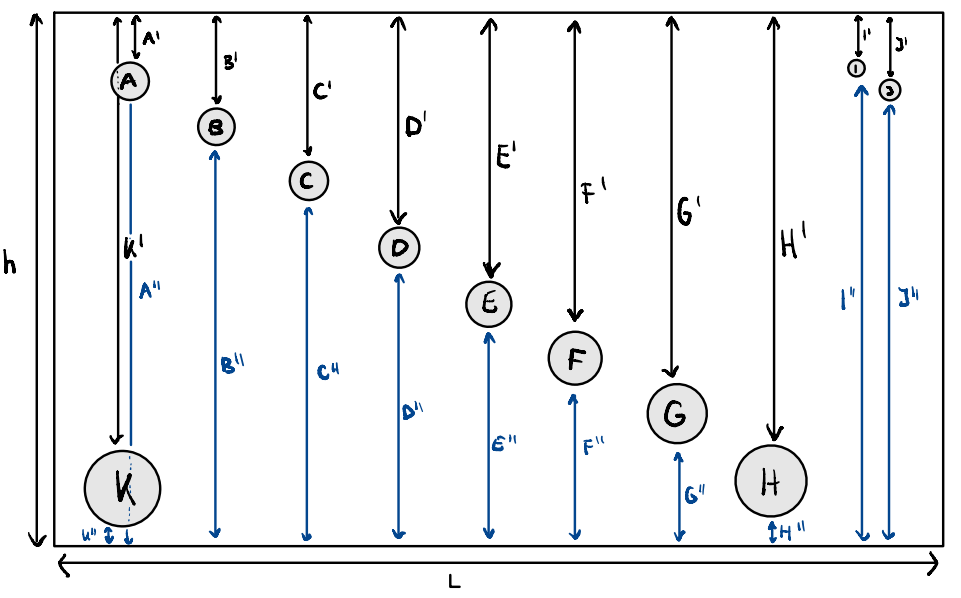
\includegraphics[width=0.8\textwidth]{bilderlit/skizze.png}
    \caption{Schematische Skizze des verwendeten Acrylblocks mit Fehlstellen $A$ bis $K$.} 
    \label{fig:skizzeyo}
\end{figure}

Die Länge $L$, Höhe $h$ und Tiefe $t$ des Acrylblocks wurden ebenfalls über die Schieblehre mit einer Ableseungenauigkeit von $\SI{0.1}{\milli\meter}$
bestimmt und sind in Tabelle \ref{tab:ausmessunggrob} angegeben.

\begin{table}
    \centering
    \caption{Allgemeine Ausmessungen des Acrylblocks mit einer Schieblehre.}
    \label{tab:ausmessunggrob}
    \begin{tabular}{c c c}
        \toprule
        Länge  $L$ [$\si{\milli\meter}$] & Höhe $h$ [$\si{\milli\meter}$]& Tiefe $t$ [$\si{\milli\meter}$] \\
        \midrule
        $\SI{150.35(10)}{}$ & $\SI{80.35(10)}{}$ & $\SI{40.30(10)}{}$ \\
        \bottomrule
    \end{tabular}
\end{table}

\subsection{Messungen am Augenmodell}

Der zweite Versuchsteil besteht aus der Untersuchung eines Augenmodells mit mehreren Grenzübergängen. Diese lassen sich gut an der Abbildung \ref{fig:augeyo} erkennen. Wie zuvor wird auf das Augenmodell Ultraschallgel aufgetragen, damit möglichst wenig
Ultraschall von der Luft absorbiert wird. Wieder wird mit der Impuls-Echo-Methode die Laufzeit $\increment t$, sowie die Spannung $U$, zwischen den zu erkennenden Peaks im \enquote{A-Scan}-Programm notiert. Es muss stets darauf geachtet werden, dass
nicht zu viel Druck auf die Oberfläche des Modells ausgewirkt wird, da sonst Risse entstehen können. Da die Ultraschallmessung sehr sensibel ist, wird darauf geachtet, dass die zu erwartenden Peaks sichtbar sind. Anhand Abbildung \ref{fig:augeyo} lassen sich
neben der ausgehenden Spannungamplitude vier weitere Peaks erwarten, da es insgemsamt vier verschiedene Grenzübergänge/Reflexionsmöglichkeiten gibt.

\begin{figure}
    \centering
    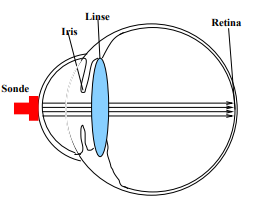
\includegraphics[width=0.5\textwidth]{bilderlit/augeyo.png}
    \caption{Schematische Skizze des verwendeten Augenmodells \cite{skript}.} 
    \label{fig:augeyo}
\end{figure}
